\documentclass[10pt,a4paper,onecolumn]{article}
\usepackage{graphicx}
\usepackage{subcaption}
\usepackage{color}
\usepackage{amsmath}
\usepackage[table]{xcolor}

\begin{document}
	\title{Logic Gates}
	\author{Nkechi Grace Okoacha}
	\maketitle
\tableofcontents
	
\newpage
\section{Introduction}
\label{intro}
	\begin{itemize}
		\item A logic gate is a building block of a digital circuit which is at the heart of any computer operation. \\
		
	\begin{center}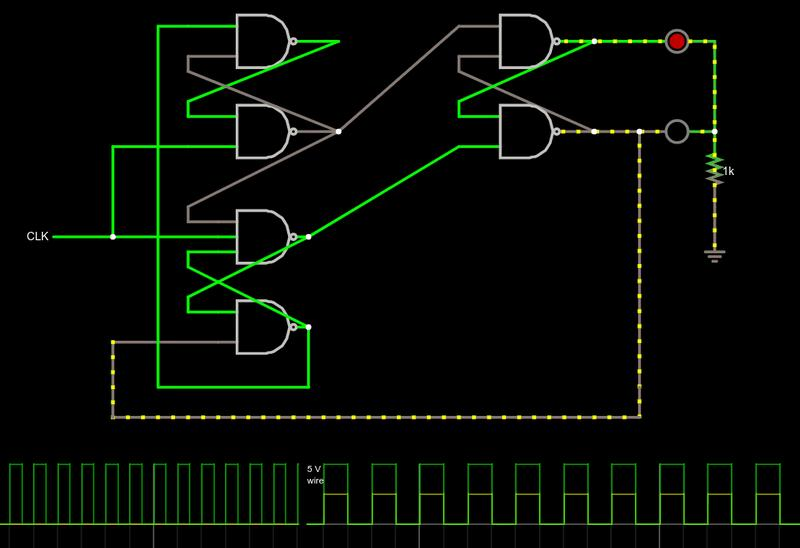
\includegraphics[width=5cm]{gst1.jpg}\end{center}
		
		\item Behind every digital system is a logic gate. \\
		
		\begin{center}
\includegraphics[width=5cm]{gst2.jpg}\end{center}
		
		\item Logic gates perform logical operations that take binary input (0s and 1s) and produce  a single binary output. They are used in most electronic device including: \\
			\begin{figure}[h!]
				\centering
				\begin{subfigure}[b]{0.2\linewidth}
				
\includegraphics[width=\linewidth]{picture1.jpg}
				\caption{Smartphones}
				\end{subfigure}
			\begin{subfigure}[b]{0.2\linewidth}
				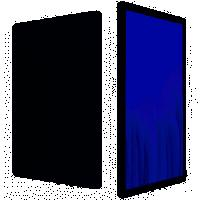
\includegraphics[width=\linewidth]{picture2.jpg}
				\caption{Tablets}
			\end{subfigure}
		\begin{subfigure}[b]{0.2\linewidth}
			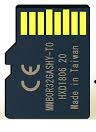
\includegraphics[width=\linewidth]{picture3.jpg}
			\caption{Memory devices}
		\end{subfigure}
			\end{figure} 
		
		\item Now think of a logic gate like a light switch, it is either in an ON or OFF position. Similarly, the input output terminals are always in one of two binary positions false(0) and true(1). Each gate has its own logic or set of rules that determines how it acts based on multiple inputs outlined in a truth table. \\
		
		\item Combining 10s, 1000s or millions of logic gates makes it possible for a computer to perform highly complex operations and tasks at ever increasing speeds. \\
		
		\item A gate is a basic electronic circuit which operates on one or more signals to produce an output signal. 
		Logic gates are digital circuits constructed from diodes, transistors, and resistors connected in such a way that the circuit output is the result of a basic logic operation (OR, AND, NOT) performed on the inputs. \\
		
		\item Fundamental gates are \color{red}AND, OR \color{black}and \color{red}NOT \\
		\begin{center}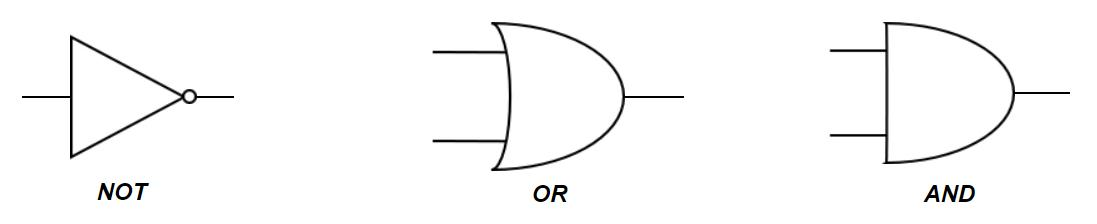
\includegraphics[width=10cm]{gst3.jpg}\end{center}
		
		\color{black}Derived Gates are \color{red}NAND, NOR, XOR \color{black}and \color{red}XNOR \color{black}(derived from the fundamental gates)
		
		Universal Gates are \color{red}NAND \color{black} and \color{red}NOR \color{black}gates (the fundamental logic gates can be realized through them).
		
		
	\end{itemize}
\section{Logic Gates}

\subsection{AND Gate}
The expression C = A X B reads as “C equals A AND B“ 
The multiplication sign (X) stands for the AND operation, same for ordinary multiplication of 1s and 0s.\\
\begin{center}
\includegraphics{gst4}\end{center}

The AND operation produces a true output (result of 1) only for the single case when all of the input variables are 1 and a false output (result of 0) where one or more inputs are 0. \\
\begin{table}[h!]
	\begin{center}
		\begin{tabular}{c|c|c}
			\textbf{A} & \textbf{B} &
			\textbf{C = A x B}\\
			\hline
			1 & 1 & 1\\
			\hline
			1 & 0 & 0\\
			\hline
			0 & 1 & 0\\
			\hline
			0 & 0 & 0\\
			\hline
		\end{tabular}
	\end{center}
\end{table} \\
\begin{center}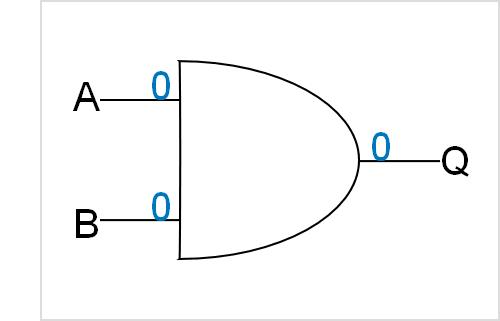
\includegraphics[width=5cm]{gst6}\end{center} 

\subsection{OR Gate}
The expression C = A + B reads as “C equals A OR B". It is the inclusive “OR”
The Addition (+) sign stands for the OR operation. \\
\begin{center}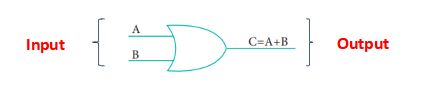
\includegraphics{gst7}\end{center}

The OR operation produces a true output (result of 1) when any of the input variable is 1 and a false output (result of 0) only when all the input variables are 0. \\
\begin{table}[h!]
	\begin{center}
		\begin{tabular}{c|c|c}
			\textbf{A} & \textbf{B} &
			\textbf{C = A + B}\\
			\hline
			1 & 1 & 1\\
			\hline
			1 & 0 & 1\\
			\hline
			0 & 1 & 1\\
			\hline
			0 & 0 & 0\\
			\hline
		\end{tabular}
	\end{center}
\end{table} \\ 
\begin{center}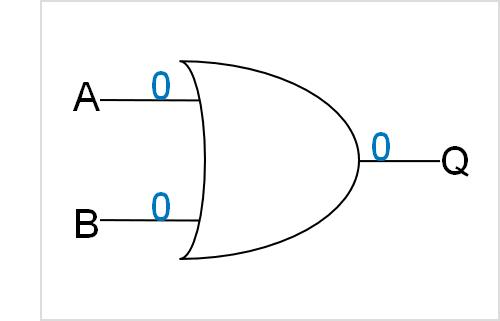
\includegraphics[width=5cm]{gst9} \end{center}

\subsection{NOT Gate}
The NOT gate is called a logical inverter. \\
It has only one input. It reverses the original input (A) to give an inverted output C. \\

\color{red}C = NOT A or C = \\ \color{black}
\begin{center}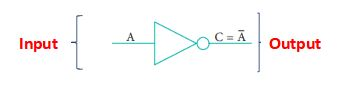
\includegraphics{gst10}\end{center}
\begin{table}[h!]
	\begin{center}
		\begin{tabular}{c|c}
			\textbf{A} & 
			\textbf{C = $\overline{A}$}\\
			\hline
			1 & 0 \\
			\hline
			0 & 1 \\
			\hline
		\end{tabular}
	\end{center}
\end{table} 
\begin{center}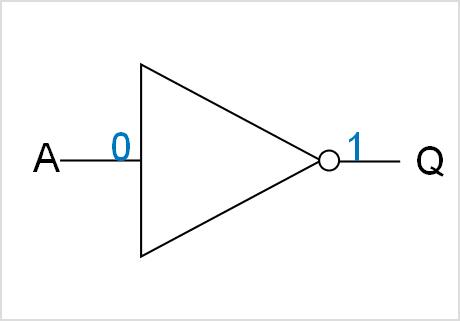
\includegraphics[width=5cm]{gst12}\end{center}

\subsection{NOR Gate}
The NOR (NOT OR) gate circuit is an inverter OR gate. \\

\color{red}Reads as C = NOT of A or B \\ \color{black}

C = \begin{center}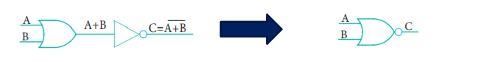
\includegraphics{gst13}\end{center}

The NOR Gate gives a true output (result of 1) only when both inputs are false (0) \\
\begin{table}[h!]
	\begin{center}
		\begin{tabular}{c|c|c|c}
			\textbf{A} & \textbf{B} &
			\textbf{A + B} & \textbf{C = $\overline{A + B}$}\\
			\hline
			1 & 1 & 1 & 0 \\
			\hline
			1 & 0 & 1 & 0 \\
			\hline
			0 & 1 & 1 & 0\\
			\hline
			0 & 0 & 0 & 1\\
			\hline
		\end{tabular}
	\end{center}
\end{table} \\


\color{red}The NOR Gate is a universal gate because it can be used to form any other kind of gate. \\ \color{black}
\begin{center}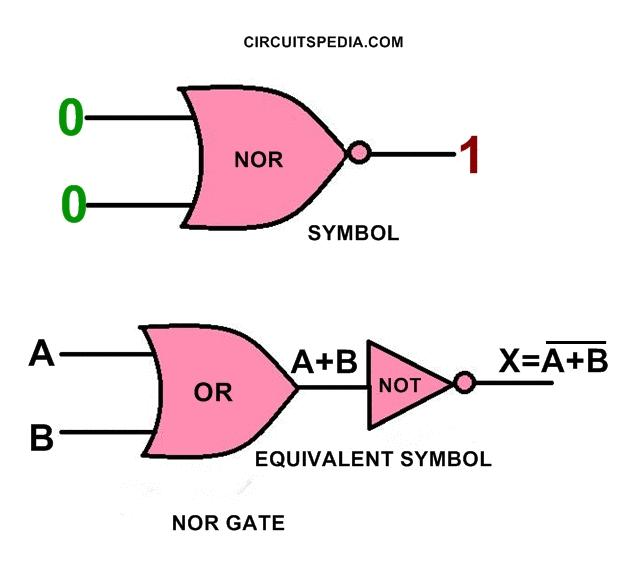
\includegraphics[width=6cm]{gst15}\end{center}

\subsection{NAND Gate}
The NAND (NOT AND) Gate is an inverted AND Gate \\
C = \begin{center}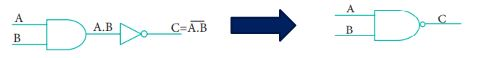
\includegraphics{gst16}\end{center}
\color{red}Reads as C = NOT of A AND B \\ \color{black}

The NAND Gate gives a false output (result of 0) only when both inputs are true (1) \\

\begin{table}[h!]
	\begin{center}
		\begin{tabular}{c|c|c|c}
			\textbf{A} & \textbf{B} &
			\textbf{A . B} & \textbf{C = $\overline{A . B}$}\\
			\hline
			1 & 1 & 1 & 0\\
			\hline
			1 & 0 & 0 & 1\\
			\hline
			0 & 1 & 0 & 1\\
			\hline
			0 & 0 & 0 & 1\\
			\hline
		\end{tabular}
	\end{center}
\end{table} 

\color{red}The NAND Gate is a universal gate because it can be used to form any other kind of gate. \\ \color{black}
\begin{center}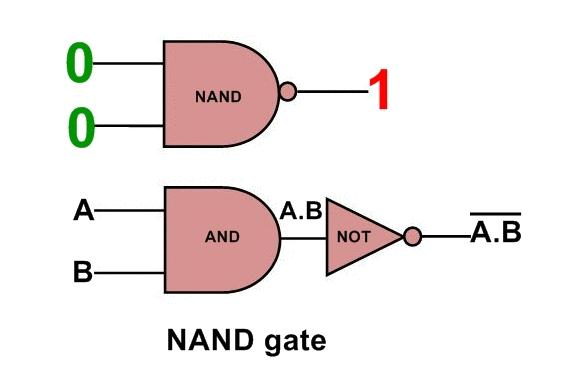
\includegraphics[width=8cm]{gst18}\end{center}

\subsection{XOR Gate}
An XOR (exclusive OR) gate acts in the same way as the exclusive OR logical connector. \\
It gives a true output (result of 1) if one, and only one, of the inputs to the gate is true (1), i.e either or but not both \\
\color{red}$\\ c = \overline{A}.B + \overline{B}.A$ \\ \color{black}
\begin{center} 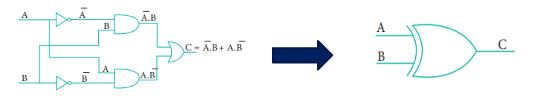
\includegraphics[width=8cm]{gst19}\end{center}
\begin{table}[h!]
	\begin{center}
		\begin{tabular}{c|c|c|c|c|c|c}
			\textbf{A} & \textbf{B} & \textbf{$\overline{A}$} & \textbf{$\overline{B}$} & \textbf{$\overline{A}$ . B} & \textbf{$\overline{B}$ . A} & \textbf{$\overline{A}$ . B} + \textbf{$\overline{B}$ . A}\\
			\hline
			1 & 1 & 0 & 0 & 0 & 0 & 0\\
			\hline
			1 & 0 & 0 & 1 & 0 & 1 & 1\\
			\hline
			0 & 1 & 1 & 0 & 1 & 0 & 1\\
			\hline
			0 & 0 & 1 & 1 & 0 & 0 & 0\\
			\hline
		\end{tabular}
	\end{center}
\end{table} 
\color{red}It uses a combination of three basic gates – AND, OR and NOT. \\ \color{black}

\subsection{XNOR Gate}
The XNOR (exclusive - NOR) gate is a combination XOR gate followed by an inverter. \\
 It is represented by the \color{red} c = $\overline{A.B} + \overline{B.A}$  \\ \color{black} \\
\begin{center}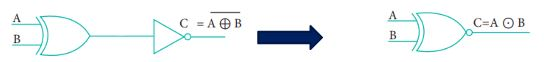
\includegraphics[width=8cm]{gst21}\end{center}
Its gives a  true output (1), if the inputs are the same, and a false output (0) if the inputs are different. \\
\begin{table}[h!]
	\begin{center}
		\begin{tabular}{c|c|c|c|c|c|c|c}
			\textbf{A} & \textbf{B} & \textbf{$\overline{A}$} & \textbf{$\overline{B}$} & \textbf{$\overline{A}$ . B} & \textbf{$\overline{B}$ . A} & \textbf{A} + \textbf{B} & \textbf{$\overline{A + B}$}\\
			\hline
			1 & 1 & 0 & 0 & 0 & 0 & 0 & 1\\
			\hline
			1 & 0 & 0 & 1 & 0 & 1 & 1 & 0\\
			\hline
			0 & 1 & 1 & 0 & 1 & 0 & 1 & 0\\
			\hline
			0 & 0 & 1 & 1 & 0 & 0 & 0 & 1\\
			\hline
		\end{tabular}
	\end{center}
\end{table} \\

\subsection{Logic Gates and their Truth Tables}
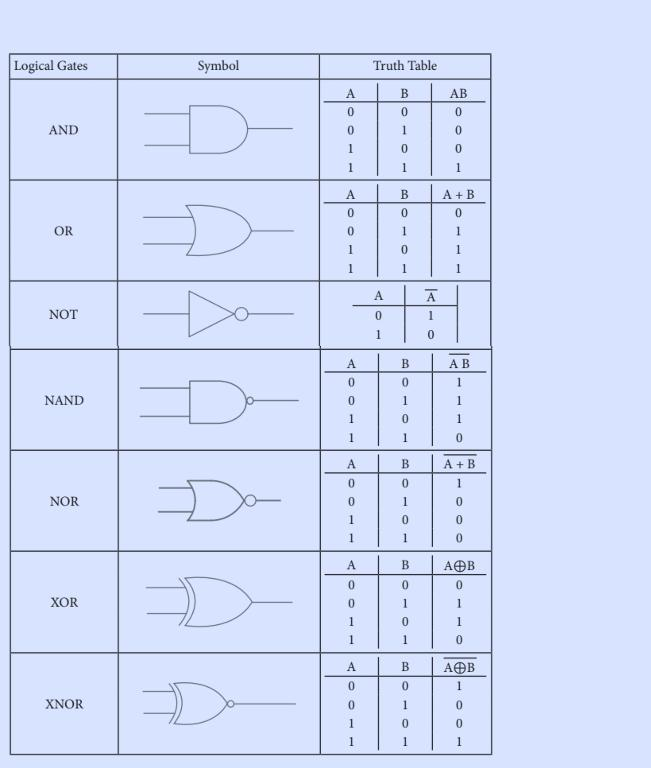
\includegraphics{gst23}

\section{Summary}
\begin{itemize}
	\item Using different combination of logic gates, complex operations can be performed. 
	\item With the Universal logic gates - NAND and NOR, any other gate can be built
	\item There is no limit to the number of gates that can be arranged together in a single device. 
	\item However, in practice, there is a limit to the number of gates that can be packed into a given physical space. 
	\item Arrays of logic gates are found in digital integrated circuits.
	\item The logic gates are abstract representations of real electronic circuits
	\item In computers, Logic gates are built using transistors combined with other electrical components like resistors and diodes. 
	\item These electrical components are wired together in order to transform a particular input to give a desired output. \cite{mygst108}
\end{itemize}

\section{Quiz}
\begin{itemize}
	\item What is the output of an AND gate if the inputs are 1 and 0?
	\item Explain the difference between the AND gate and the OR gate.
	\item What is the output of a NOT gate if the inputs is 0?
	\item Which logic gate is this?
	\item Which gate is also known 
	a logical converter?
\end{itemize}

\centering
\includegraphics[width=10cm]{gst24}

\newpage
\bibliographystyle{ieeetr}
\bibliography{gst108}
\end{document}